% Revised VE Simulation Report
% Arseniy Khvorov
% Created 2019/06/04
% Last edit 2019/06/04

\documentclass[11pt]{article}

\usepackage[utf8x]{inputenc}

%%% PAGE DIMENSIONS
\usepackage{geometry}
\geometry{a4paper}
\geometry{margin=1in} % for example, change the margins to 2 inches all round

\usepackage{graphicx} % support the \includegraphics command and options

\usepackage[parfill]{parskip} % Begin paragraphs with an empty line rather than an indent

%%% PACKAGES
\usepackage{booktabs} % for much better looking tables
\usepackage{array} % for better arrays (eg matrices) in maths
\usepackage{paralist} % very flexible & customisable lists (eg. enumerate/itemize, etc.)
\usepackage{verbatim} % adds environment for commenting out blocks of text & for better verbatim
\usepackage{subfig} % make it possible to include more than one captioned figure/table in a single float
\usepackage{float}

\usepackage[numbers]{natbib}
\bibliographystyle{vancouver}


\usepackage{multicol}
\usepackage{multirow}
\usepackage{xcolor}
\usepackage{amsmath}

\usepackage[T1]{fontenc}
\usepackage{lmodern}

%%% FLOWCHART
\usepackage{tikz} % flowcharts
\usetikzlibrary{shapes.geometric, arrows, positioning, backgrounds}


\renewcommand{\arraystretch}{1.1}

%%% HEADERS & FOOTERS
\usepackage{fancyhdr} % This should be set AFTER setting up the page geometry
\pagestyle{fancy} % options: empty , plain , fancy
\renewcommand{\headrulewidth}{0pt} % customise the layout...
\lhead{\leftmark}\chead{}\rhead{\rightmark}
\lfoot{}\cfoot{\thepage}\rfoot{}

%%% SECTION TITLE APPEARANCE
\usepackage{sectsty}
\allsectionsfont{\sffamily\mdseries\upshape} % (See the fntguide.pdf for font help)
% (This matches ConTeXt defaults)

%%% ToC (table of contents) APPEARANCE
\usepackage[nottoc,notlof,notlot]{tocbibind} % Put the bibliography in the ToC
\usepackage[titles,subfigure]{tocloft} % Alter the style of the Table of Contents
\renewcommand{\cftsecfont}{\rmfamily\mdseries\upshape}
\renewcommand{\cftsecpagefont}{\rmfamily\mdseries\upshape} % No bold!

\usepackage[bookmarks,hidelinks]{hyperref}

%%% END Article customizations

%%% The "real" document content comes below...

\title{VE estimates with administrative data}
\author{Arseniy Khvorov}
\date{October 2019} 

\begin{document}
\maketitle

\renewcommand{\abstractname}{}
\begin{abstract}
	\begin{center}
	Simulation repository\\
	https://github.com/khvorov45/ve-admin
	\end{center}
\end{abstract}

\tableofcontents

\pagebreak

%
\section{Methods}

%%
\subsection{Core simulation}

Starting population was the general population. Its size was set to 500,000. Every individual had their attributes randomly allocated in the order shown in Figure \ref{SimDiag} and with probabilities shown in tables below.

First allocated attribute was true vaccination status. Measurement of this status for the purposes of the simulated study was allowed to be inaccurate in order to simulate exposure miscalssification. True vaccination status was used to determine which probability to use to allocate individuals to the flu-infected category. Both vaccinated and unvaccinated subjects were allocated to the non-flu infected category with the same probability. The remaining subjects ended up as part of the non-ARI category.

Everyone with an ARI (either infected with flu or a non-flu pathogen) was assigned to either the symptomatic or the asymptomatic group. Those who were symptomatic were assigned to the clinically assessed or unassessed groups. Being clinically assessed in this context means that they presented to a clinic with ARI illness and they were classified as an ARI case. These clinically assessed ARI cases got one probability of being tested, everyone else got another. Tests were allowed to be imperfect to simulate outcome misclassification.

%%
\subsection{Population summary}

Each population was collapsed down to summary results - each individual was considered to be part of one of eight categories: administrative/surveillance vaccinated/unvaccinated case/control as shown in Figure \ref{PopAgg}.

\begin{figure}[h]
	\centering
		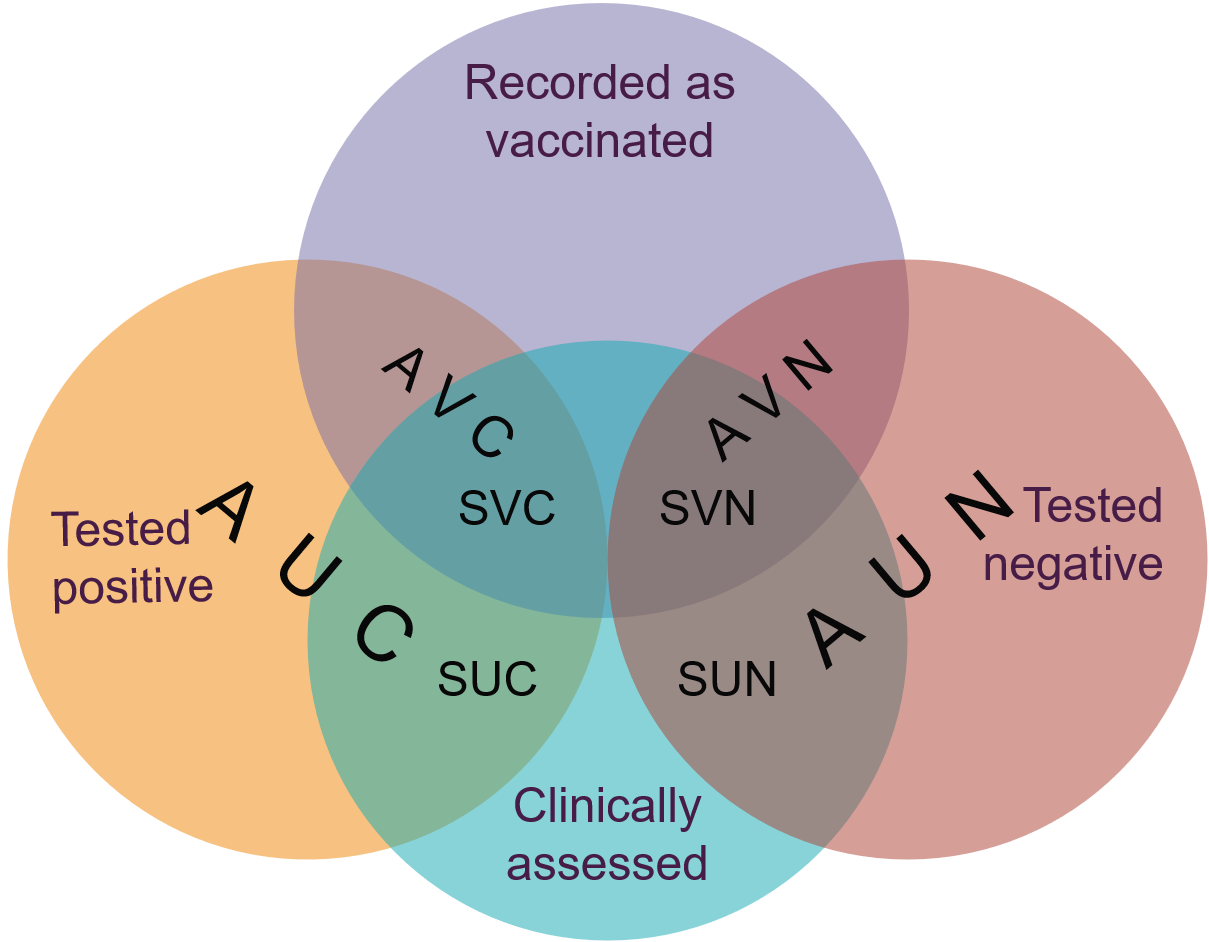
\includegraphics[width=0.5\linewidth]{../sim-diag/popagg-venn.png}
		\caption{
Assignment of an individual to appropriate categories. A - administrative, S - surveillance, V - vaccinated, U - unvaccinated, C - case, N - non-case (control). \label{PopAgg}
		}
\end{figure}

Individuals in each of the categories were counted. These counts were representative of those that could have been obtained if a test-negative study was done on that population either using administrative or surveillance data. VE estimates could then be calculated as 1 - OR where OR = $\frac{\text{Odds in vaccinated}}{\text{Odds in unvaccinated}}$ where Odds = $\frac{\text{Count of cases}}{\text{Count of controls}}$.

\pagebreak

\begin{figure}[H]
	\centering
		\tikzstyle{group} = [rectangle, minimum width=3cm, minimum height=1cm, text centered, text width=3cm, draw=black, fill=black, text=white, fill opacity=0.9, text opacity=1]

\tikzstyle{arrowlab} = [rectangle, fill=black, text=white, fill opacity = 0.9]

\tikzstyle{arrow} = [thick, ->, >=stealth]

\pgfdeclarelayer{bg}
\pgfsetlayers{bg, main}

\begin{tikzpicture}[node distance=2cm]
\node (pop) [group] {Population};
\node (truevac) [group, below of=pop, left of=pop] {True vaccinated};
\node (trueunvac) [group, below of=pop, right of=pop] {True unvaccinated};
\node (recvac) [group, below of=truevac] {Recorded as vaccinated};
\node (recunvac) [group, below of=trueunvac] {Recorded as unvaccinated};
\node (nonflu) [group, below of=recunvac, left of=recunvac] {Non-flu};
\node (nonari) [group, below left=1cm and 1cm of nonflu] {Non-ARI};
\node (flu) [group, right=1cm of nonflu] {Flu};
\node (ari) [group, below of=flu, left of=flu] {ARI};
\node (sympt) [group, below of=ari] {Symptomatic};
\node (asympt) [group, left=1cm of sympt] {Asymptomatic};
\node (clin) [group, below of=sympt] {Clinically assessed};
\node (nonclin) [group, left=1cm of clin] {Unassessed};
\node (test) [group, below of=clin] {Tested};
\node (nontest) [group, left=1cm of test] {Not tested};
\node (fluinf) [group, below of=test] {Flu-infected};
\node (notfluinf) [group, left=1cm of fluinf] {Non flu-infected and uninfected};
\node (pos) [group, below of=fluinf] {Positive};
\node (neg) [group, left=1cm of pos] {Negative};

\draw[arrow] (pop) -- node[arrowlab] {$v$} (truevac);
\draw[arrow, dashed] (pop) -- (trueunvac);

\draw[arrow] (truevac) -- node[arrowlab] {$s_{e,v}$} (recvac);
\draw[arrow, dashed] (truevac) -- (recunvac);
\draw[arrow] (trueunvac) -- node[arrowlab] {$s_{p,v}$} (recunvac);
\draw[arrow, dashed] (trueunvac) -- (recvac);

\begin{pgfonlayer}{bg}
\draw[arrow] (truevac) -- node[arrowlab, yshift=-1cm, xshift=1.5cm] {$f(1-e)$} (flu);
\draw[arrow] (truevac) -- node[arrowlab, yshift=-1cm, xshift=0.5cm] {$l$} (nonflu);
\draw[arrow] (trueunvac) -- node[arrowlab, yshift=-1cm, xshift=0.75cm] {$f$} (flu);
\draw[arrow] (trueunvac) -- node[arrowlab, yshift=-1cm, xshift=-0.5cm] {$l$} (nonflu);
\draw[arrow, dashed] (trueunvac) -- (nonari);
\draw[arrow, dashed] (truevac) -- (nonari);

\draw[arrow, dotted] (nonari) -- (nonclin);
\end{pgfonlayer}

\draw[arrow, dotted] (nonflu) -- (ari);
\draw[arrow, dotted] (flu) -- (ari);

\draw[arrow] (ari) -- node[arrowlab] {$p$} (sympt);
\draw[arrow, dashed] (ari) -- (asympt);

\draw[arrow] (sympt) -- node[arrowlab] {$c$} (clin);
\draw[arrow, dashed] (sympt) -- (nonclin);

\draw[arrow, dotted] (asympt) -- (nonclin);

\draw[arrow] (clin) -- node[arrowlab] {$t_a$} (test);
\draw[arrow, dashed] (clin) -- (nontest);
\draw[arrow] (nonclin) -- node[arrowlab, yshift=-0.2cm, xshift=0.5cm] {$t_n$} (test);
\draw[arrow, dashed] (nonclin) -- (nontest);

\draw[arrow] (test) -- (fluinf);
\draw[arrow, dashed] (test) -- (notfluinf);

\draw[arrow] (fluinf) -- node[arrowlab] {$s_e$} (pos);
\draw[arrow, dashed] (fluinf) -- (neg);
\draw[arrow] (notfluinf) -- node[arrowlab] {$s_p$} (neg);

\end{tikzpicture}
		\caption{
Simulation decision tree. Parameter key is in Table \ref{TabParKey}. Solid lines mean allocation with probabilities represented by the indicated parameters. Dashed line probabilities are complements of corresponding solid line probabilities. Dotted lines represent full-group allocation. Probability of being flu-infected for those who are tested isn't indicated because it wasn't necessary for the purposes of simulations. \label{SimDiag}
		}
\end{figure}

\pagebreak
%%
\subsection{Parameter Variation}

Every parameter in the simulation was set at a prespecified value. Some of the parameters were set to vary (their prespecified value would have been ignored then). Setting a parameter to vary meant meant that the parameter was assigned a small set of values, set to the first of those values, a set amount of populations were simulated using that value, then it was set to the next value and so on until the simulation went through the entire set.

If multiple parameters were set to vary the simulation would have gone through all possible combinations of all parameters values.

%%
\subsection{Mixed-group simulations}

If a simulation required a population to be composed of multiple groups, each group was simulated as if it were a separate population. The only mixed combination used was children/adults/elderly. The total size of each group was obtained by multiplying the total requested sample size (usually 200,000) by the specified proportion of each group in the population (this is the $w$ parameter which would have been set to 1 if there was only one group in the population). Amounts of cases and controls were counted in each of the groups and added together to represent the counts obtained from the full population.

%%
\subsection{Additional simulations}

To determine the effects of individual parameters, an additional set of simulations was performed with parameters fixed to values shown in Table \ref{AddSim}. This set of parameter values produced unbiased VE estimates in surveillance data. Using this as a baseline, required parameters could be varied (e.g. $s_p$ can be set below 1) to observe their effect in absence of other sources of bias. Additional simulations were also used to observe the effect some parameters have on others (e.g. how $s_p$ set below 1 affects variation of VE estimates at different values of $t_n$).

\pagebreak
%%
\subsection{Parameter estimates used}

\begin{table}[h]
\centering
\caption{
Parameter names, meanings and values used in simulations. "Range used" shows the range of values used for variation in individual age group simulations. Tables \ref{TabComb} contains values and patterns used for variation in mixed group simulations. Every parameter except $c$ represents an absolute probability (some of them only apply to subsets of the population). Only relative probability estimates could be obtained for $c$ (by comparing presentation counts found in ASPREN data \cite{ASPREN} to expected underlying population size derived from other parameter estimates), its values were  set to 1 in individual group simulations unless it is the parameter varied. Parameter $w$ was only relevant if the population was requested to be composed of multiple groups. Shown values are the ones used in children/adults/elderly mixed simulation. In individual simulations, $w$ was set to 1. Estimates of $v$ and $e$ were derived from provided data. \label{TabParKey}
}
	% Table generated by Excel2LaTeX from sheet 'ParEstUsedInd'
\begin{tabular}{cp{13.285em}>{\centering}p{4.57em}cccc}
\toprule
\textnormal{Par.} & \multicolumn{1}{c}{Description} & Range Used & \multicolumn{1}{p{4.215em}}{Children (<15)} & \multicolumn{1}{p{4.07em}}{Adults (15-65)} & \multicolumn{1}{p{3.5em}}{Elderly (65+)} & Ref. \\
\midrule
$w$  & Proportion of the age groups in the general population &  & 0.189 & 0.657 & 0.154 & \cite{ABSDemo} \\
$v$ & Probability of being vaccinated & 0.05 - 0.5 & 0.1  & 0.25  & 0.66 &  \\
$s_{e,v}$ & Sensitivity of exposure measurement & 0.9 - 1 & 0.9  & 0.95  & 0.98 & \cite{Irving;2009, Donald;1999, Rolnick;2013} \\
$s_{p,v}$ & Specificity of exposure measurement & 0.5 - 1 & 0.9  & 0.8  & 0.7 & \cite{Irving;2009, Donald;1999, Rolnick;2013} \\
$e$    & Vaccine effectiveness & 0.1 - 0.9 & 0.6  & 0.5  & 0.4 & \\
$f$ & Influenza risk in unvaccinated & 0.05 - 0.15 & 0.15  & 0.08  & 0.05 & \cite{Tokars;2017} \\
$l$ & Non-influenza ARI risk in vaccinated and unvaccinated & 0.1 - 0.3 & 0.3   & 0.15  & 0.1 & \cite{ADH2017, ADH2018} \\
$p$ & Probability of the ARI being symptomatic & 0.1 - 0.9 & 0.84  & 0.84  & 0.84 & \cite{Leung;2015} \\
$c$ & Relative probability of being clinically assessed as having ARI when it is symptomatic & 0.1 - 0.9 & 0.4 & 0.3 & 1 & \\
$t_a$ & Tested probability for clinically assessed ARI & 0.1 - 0.9 & 0.17  & 0.35  & 0.22 & \cite{ASPREN} \\
$t_n$ & Tested probability for everyone without clinically assessed ARI & 0 - 0.3 & 0.15  & 0.15  & 0.15 & \\
$s_e$ & Sensitivity of influenza test & 0.5 - 1 & 0.86  & 0.86  & 0.86 & \cite{Druce;2004} \\
$s_p$ & Specificity of influenza test & 0.9 - 1 & 0.984 & 0.984 & 0.984 & \cite{Druce;2004} \\
\bottomrule
\end{tabular}%

\end{table}

\pagebreak



\cite{ASPREN}

\pagebreak
\thispagestyle{plain}
\bibliography{references}

\end{document}
